\section{函数-上}\label{003}

\begin{flushright}{\kaishu 天地之间\ 人居其一\ 连接天地\ 类于万物\ 象以形分\ 形以名别}\end{flushright}

\begin{tcolorbox}[size=fbox, breakable, enhanced jigsaw, title={函数 (function)}]

听到``function'', 第一反应可能是``方程'', 事实上函数才是 function,
方程或者等式应该叫做 equation. 不细想可能会觉得他们差别不大,
不过等式通常是来解未知的, 而函数通常是用来描述两个变量之间的关系.

非正式的, 初中阶段类似 $y=ax+b$
形式的一次函数可能是大家接触到的比较早的一个函数的例子. 有时候也会有类似
$f(x)=ax+b$ 这种标记, 意为: 一个以 $x$ 为变量的函数;
这种标记方便之处是可以很方便的标出当 $x$ 等于某个值, 例如 $42$
时函数的取值, 即 $f(42)=42a+b$. 另外 $y=ax+b$ 也可以写成
$y(x)=ax+b$ , $y$ 作为函数, 其变量为 $x$.

传统定义, 函数通常用来描述变化过程中两个变量的关系, 若有两个变量 $x$
和 $y$, 如果对于任意一个 $x$ 都有一个唯一确定 (unique) 的 $y$
与其对应, 那么就说 $x$ 是自变量 (independent variable), $y$ 是因变量
(dependent variable). $x$ 的取值范围称为函数的\textbf{定义域}
(domain), 可能输出的 $y$ 范围称为函数的\textbf{值域} (range).

自然科学和社会科学通常会用类似下左图的形式来可视化函数,
横轴竖轴分别标记两个变量的取值范围, 通过函数图像,
便可以找到当一个变量取某个特定值时另一变量对应的值.
下右图给出了一个经济学中的例子

\begin{tcolorbox}[size=fbox, breakable, enhanced jigsaw]
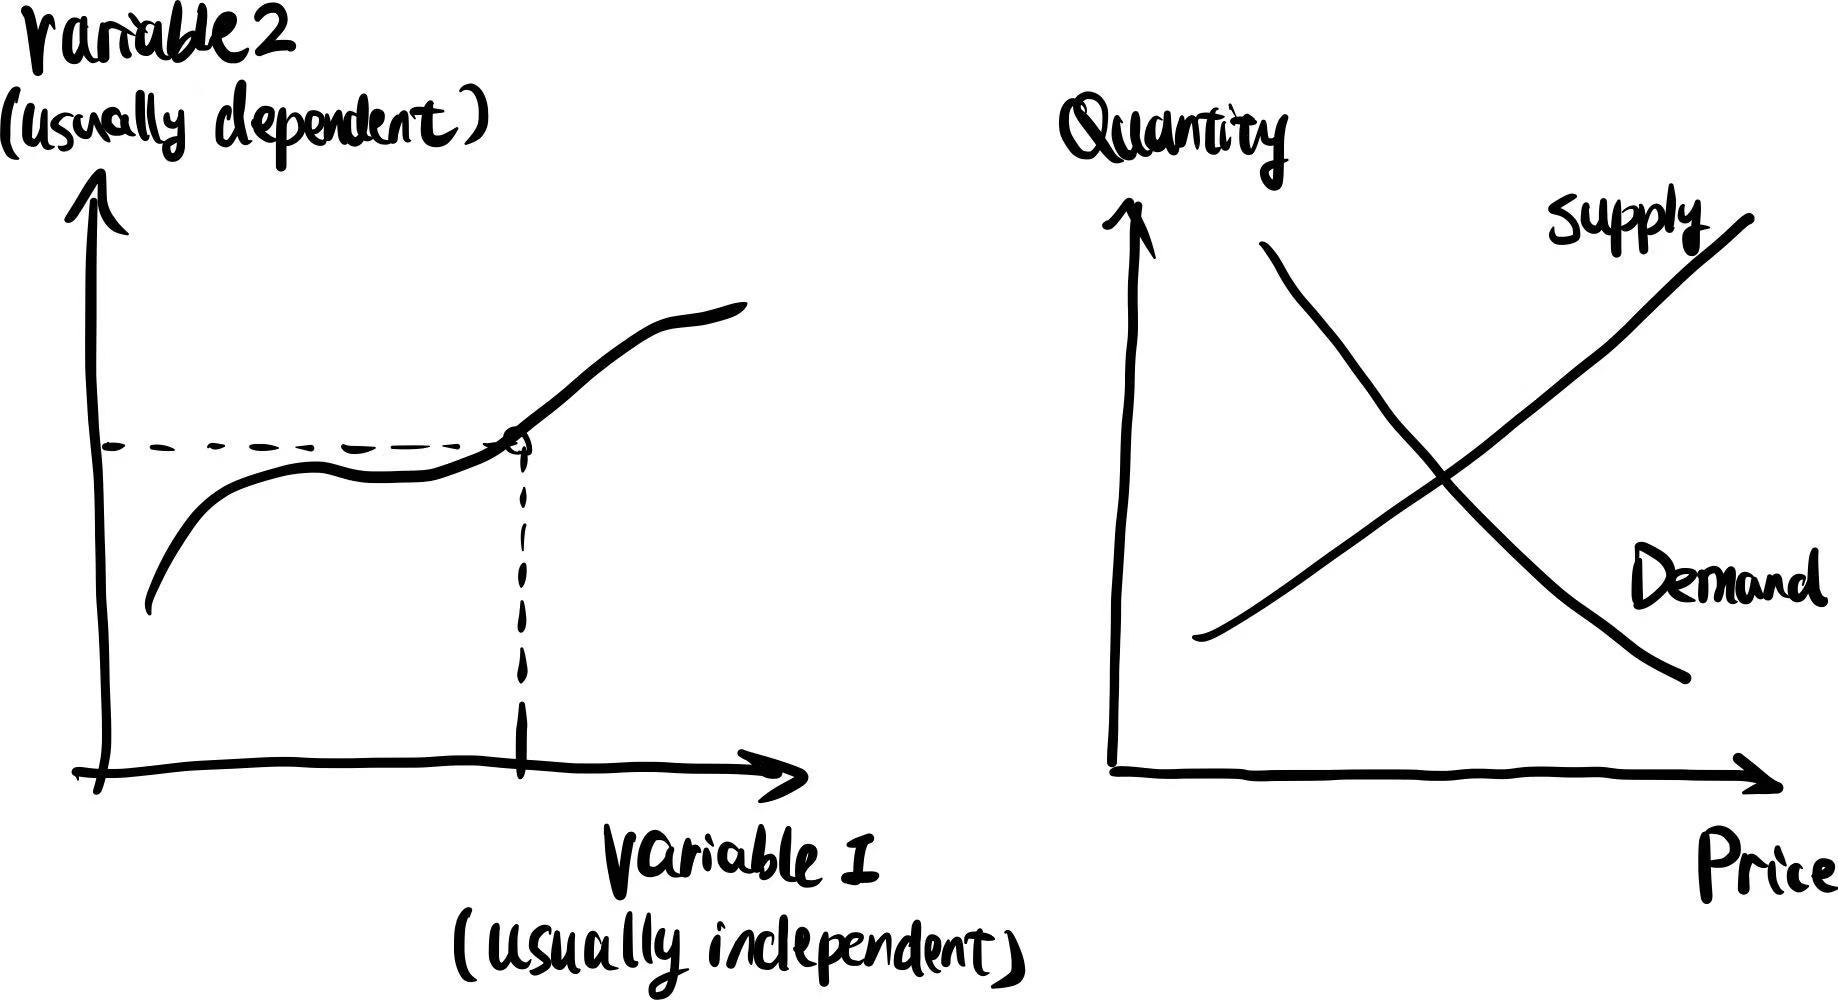
\includegraphics[width=0.9\textwidth]{img/image-20230228095149998.png}

\kaishu{\small 随着某商品的市场价格 (price) 增高, 生产者的生产意愿自然是增高的,
因为不考虑成本和其他因素变化的情况下 (Ceteris Paribus),
多生产的利润会更高, 因此供给曲线 (supply) 上扬, 反映出价格和供给量
(supply quantity) 的正相关; 另一方面,
消费者的消费意愿随着价格上涨自然是下降的, 于是需求曲线 (demand) 下压,
反映出价格和需求量 (demand quantity) 的负相关.

两条曲线分别对应着供给量和需求量关于价格的函数,
两函数的焦点反映了理想的自由市场下的最终成交价格和供需量
(因为在这个点达到了供需平衡 - equilibrium) ,
焦点向下作竖直线与横轴的焦点便显示了最终成交价格,
焦点向左作水平线与竖轴的交点便显示了平衡点的供需量.}
\end{tcolorbox}

在工程和计算机科学等思维里, 函数更像下左图所示, 给定一个输入 (input),
函数如同一台机器, 在加工后给出一个输出 (output); 这台机器非常可靠,
同样的输入能够稳定输出同样结果. 下右图给了一个例子

\begin{tcolorbox}[size=fbox, breakable, enhanced jigsaw]

\includegraphics[width=0.9\textwidth]{img/image-20230228095405809.png}

\kaishu{\small 假想有这样一个叫做``首都'' (Captital) 的函数,
放入一个国家名便会稳定输出这个国家的首都,
数学上我们可以这么标记下右图的例子 $\text{Capital(China)=Beijin}$.}
\end{tcolorbox}

函数的近现代定义和工科思维里的图景就很像, 考虑集合 $X$ 和 $Y$,
且它们不是空的, 如果存在某种特定的对应关系 $f$, 使得对于 $X$
中任意一个元素 $x$, 在 $Y$ 中都有唯一确定的元素 $y$ 和 $x$ 对应,
那么就称\textbf{映射} (mapping)\footnote{~Mapping 这个词用在这很贴切,
  map有地图的意思,
  ``映射''和地图上的每个点对应着实际区域上的一个个位置很相似.}
$f: A\rightarrow B$ 为从 $X$ 到 $Y$ 的一个函数, 记作
$y=f(x), x\in X$ 或者 $f(X)=\{y|f(x)=y, y\in Y\}$;
第一种记法强调元素的映射, 第二种记法强调整个集合的映射, $X$
在这里便是这个映射的定义域, $f(X)$ 是值域, $Y$
是这个映射的\textbf{陪域} (codomain, 也叫做上域, 到达域, 对应域),
大括号表示 $X$ 被映射到的集合, 其元素 $y$ 满足竖线后的条件, 即 $y$
是自 $x$ 通过 $f$ 这个映射得到, 并且 $y$ 属于 $Y$.
这样定义的直观感受类似下左图, 之前``首都''函数便类似下右图

\begin{tcolorbox}[size=fbox, breakable, enhanced jigsaw]
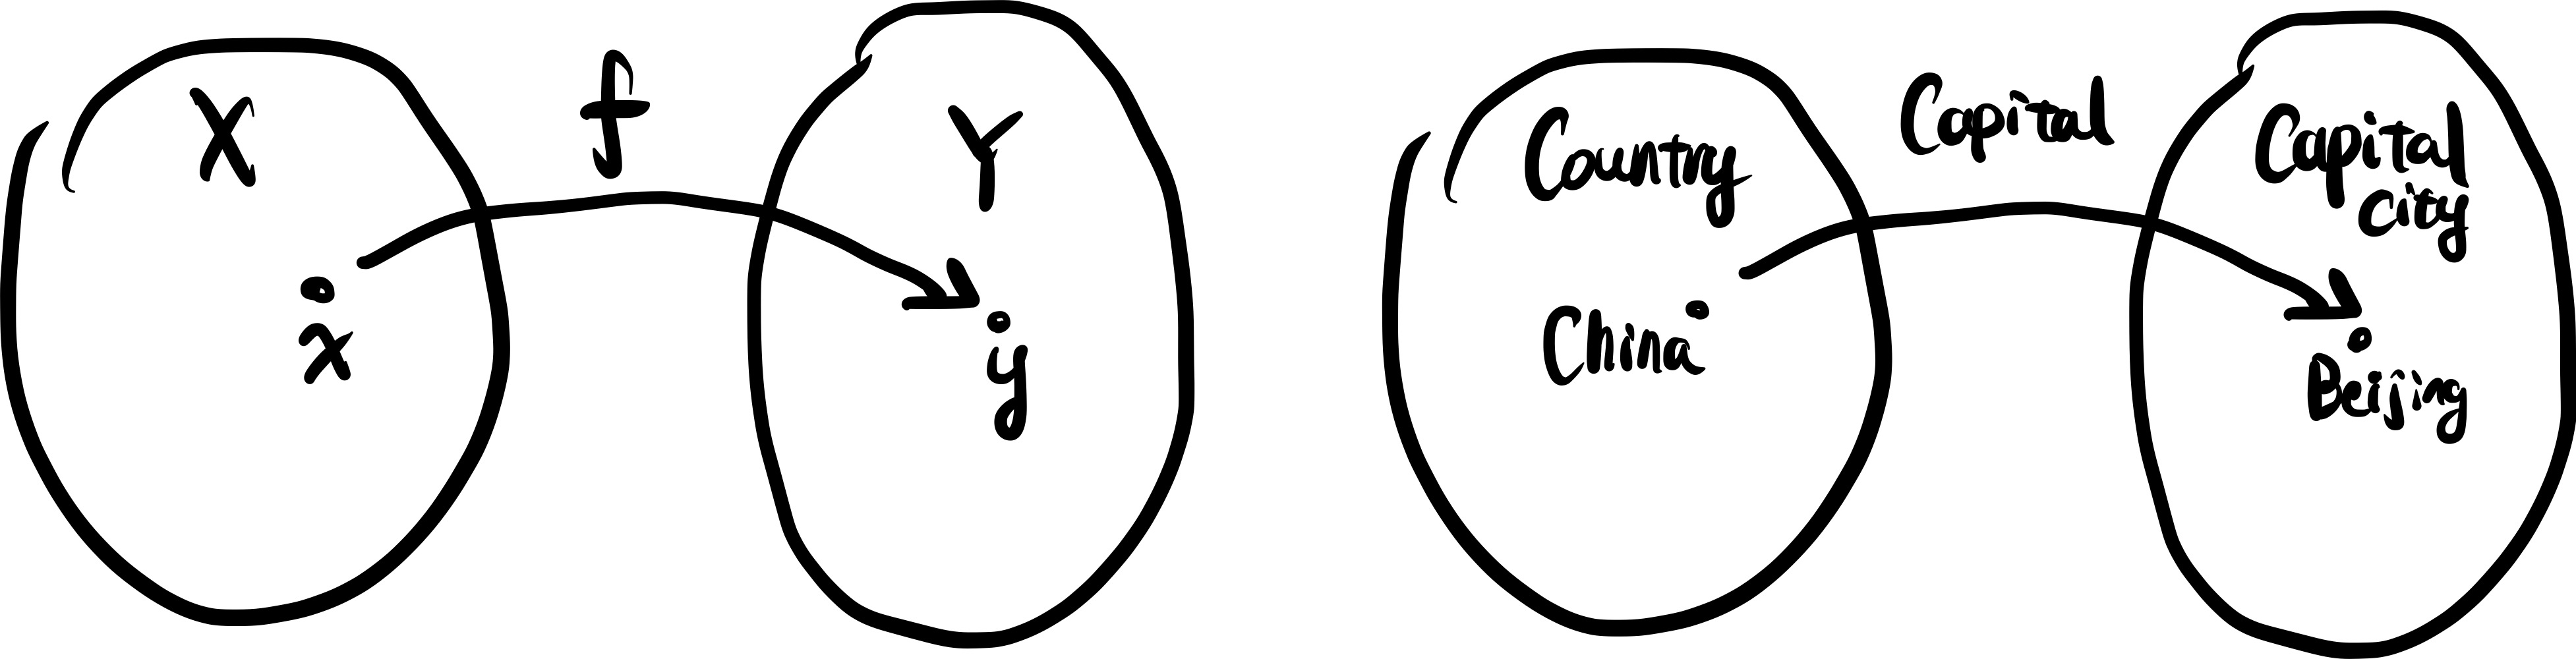
\includegraphics[width=0.9\textwidth]{img/image-20230228112941902.png}

\kaishu{\small Country这个集合里包含了很多国家, \{中国, 美国, 日本, \ldots\}; Capital
city这个集合里包含了很多城市, \{北京, 华盛顿, 东京, \ldots\};
Capital这个函数便描述了Country中的元素和Capital city中的元素的对应关系.}
\end{tcolorbox}

\end{tcolorbox}